\section{Development Workflow}

We motivate our development workflow from previous work 
\cite{PureScript2019} by extending the \fancyname{Scribble} toolchain
and generating APIs that integrate the developer's 
application logic
into the execution of the communication automata.

We visualise the workflow in \cref{fig:devworkflow} 
and provide a brief overview:

\begin{enumerate}

\item The developer supplies the communication protocol written in
\fancyname{Scribble} (\cref{subsection:scribble}), 
stating the role (hereafter \textit{endpoint})
to generate APIs for,
and the code generation \textit{target} 
(i.e. whether the role runs on the server or the web browser).

\item \fancyname{SessionTS} delegates to the 
\fancyname{Scribble} toolchain for verifying the well-formedness of
the protocol and expects to receive a DOT graph representation of
the endpoint FSM (\cref{subsection:efsm}). 
\fancyname{SessionTS} parses the endpoint's 
interactions from the DOT graph and generates TypeScript APIs
for the developer (\cref{subsection:apigen}) 
tailored to the specified target.

\item The developer implements their web application using the
generated APIs. Implementations that pass the type-checking phase
of the TypeScript Compiler are guaranteed to be free from 
communication errors by session type theory.

\end{enumerate}

\begin{figure}[!ht]
\centering
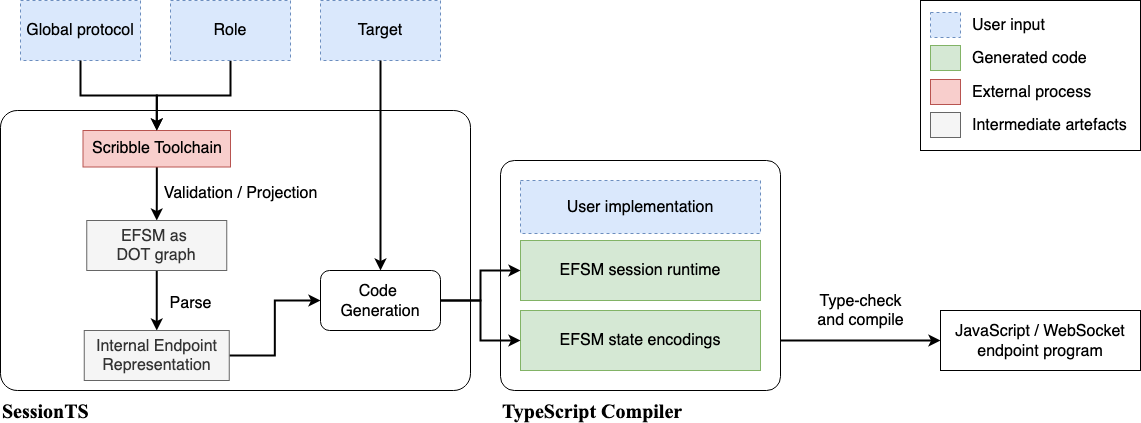
\includegraphics[width=\textwidth]{DevelopmentWorkflow}
\captionof{figure}{Overview of \fancyname{SessionTS} Development Workflow}
\label{fig:devworkflow}
\end{figure}

\subsection{Protocol Specification with \fancyname{Scribble}}
\label{subsection:scribble}

We use the \fancyname{Scribble} protocol description language, 
as presented in
\cite{Scribble}, for formalising the communication structure. This is
inspired by existing work on implementing session type theory 
in mainstream programming languages
\cite{Hybrid2016, PureScript2019, Python2017}. 
We use the variant of the \fancyname{Scribble} language 
previously introduced in \cref{subsection:bgscribble}.

\subparagraph{Type declaration statements}
Specific to our TypeScript API generation toolchain,
the developer is \textit{not} required to explicitly
add type declaration statements for built-in types.
\cref{lst:adder} is a \textit{syntactically correct}
\fancyname{Scribble} protocol as far as 
\fancyname{SessionTS} is concerned. 
Internally, \fancyname{SessionTS} inspects the protocol file
and parses existing type declarations using regular expressions
(or \textit{regex}) -- this is necessary to extract any
custom data types that will appear in the communication (for example,
\cref{lst:game}), and allows \fancyname{SessionTS} to inject
``boilerplate'' type declarations for built-in TypeScript types before
calling \fancyname{Scribble}.

\begin{figure}[!ht]
\begin{lstlisting}[language=Scribble]
module Adder;

global protocol Adder(role Client, role Svr) {
	choice at Client {
		ADD(number, number) from Client to Svr;
		RES(number)         from Svr to Client;	
	} or {
		QUIT(string) from Client to Svr;	
		TERMINATE()  from Svr to Client;
	}
}
\end{lstlisting}
\captionof{lstlisting}{The \tprotocol{Adder} Protocol}
\label{lst:adder}
\end{figure}

We will use the \tprotocol{Adder} protocol as a running example
to demonstrate how our work performs TypeScript API generation.

\subsection{From \fancyname{Scribble} to EFSM}
\label{subsection:efsm}

\begin{itemize}
\item scribble validates the protocol
\item use flag to obtain EFSM representation
\item DOT graph output
\item parse in python -- use open-source library for this
\end{itemize}

\subsection{Code Generation}
\label{subsection:apigen}

\begin{itemize}
\item api generation is a function of the EFSM representation
\item traditional methods -- visitor pattern on the EFSM and using stringbuilder to build the file
\item templating library is more suitable to decouple the ``presentation'' (how the code should look) from the ``content'' (the EFSM which is used to build the code)
\item strategy pattern to support the two required build targets (in node and react)
\end{itemize}